% 02_recombination.tex
\section{Recombination and the visibility function}
\label{ch:recomb}

The CMB exists because at some time in the universe's past, free electrons combined with protons to form neutral hydrogen, and photons that had been Thomson-scattering off those electrons suddenly found themselves in a transparent universe. This chapter computes the ionisation history $x_e(z)$ in detail, then constructs the \emph{visibility function} $g(\tau) = \dot\kappa(\tau)\, e^{-\kappa(\tau)}$ -- the probability density that a CMB photon last scattered at conformal time $\tau$. The visibility function will appear in every line-of-sight integral in chapters 4-7.

Two pieces of physics determine $x_e(z)$. At high redshift, the photon-electron-proton plasma is in thermal equilibrium and chemical equilibrium gives the Saha equation. As the universe cools, the recombination rate cannot keep up with the expansion and the system departs from equilibrium; we then need a rate equation (Peebles 1968). Helium recombines somewhat earlier and has its own structure. Modern treatments (RECFAST, CosmoRec, HyRec) refine the original Peebles equation with a careful accounting of bound-state physics; we use the RECFAST formulation, which agrees with the others to better than $0.1\%$.

\subsection{Equilibrium: the Saha equation}

In thermal equilibrium, the abundances of $e^-$, $p$, and $H$ are related by chemical-potential balance:
\[
  \mu_p + \mu_e = \mu_H.
\]
Each species has a Maxwell-Boltzmann distribution in the non-relativistic regime ($T \ll m_i c^2$):
\[
  n_i = g_i \Bigl(\frac{m_i T}{2\pi}\Bigr)^{3/2} e^{-(m_i - \mu_i)/T},
\]
with $g_i$ the internal degeneracy ($g_p = g_e = 2$, $g_H = 4$). Taking the ratio
\[
  \frac{n_e n_p}{n_H} = \frac{g_e g_p}{g_H}\, \frac{m_e m_p}{m_H}^{3/2}\, T^{3/2}\, e^{-(m_e + m_p - m_H)/T},
\]
and noting $m_e + m_p - m_H = B_H$ (the binding energy of hydrogen, $13.6\,\mathrm{eV}$) and $m_p/m_H \approx 1$,
\[
  \frac{n_e n_p}{n_H} = \Bigl(\frac{m_e T}{2\pi}\Bigr)^{3/2}\, e^{-B_H/T}.
\]
Defining the free-electron fraction $x_e = n_e/n_H^\mathrm{tot}$ and using charge neutrality $n_p = n_e$ together with conservation $n_p + n_H = n_H^\mathrm{tot}$, we obtain the Saha equation for hydrogen:
\begin{equation}
  \frac{x_e^2}{1 - x_e} = \frac{1}{n_H^\mathrm{tot}}\,\Bigl(\frac{m_e T}{2\pi}\Bigr)^{3/2}\, e^{-B_H/T}.
  \label{eq:Saha_H}
\end{equation}
The right-hand side falls exponentially when $T$ drops below $B_H$, so $x_e$ falls from $\sim 1$ to $\sim 0$ over a temperature range $\Delta T/T \sim T/B_H \sim 1/40$ near $T \approx 3000\,\mathrm{K}$ (i.e.\ $z \approx 1100$).

The same logic applies to helium. There are two ionisation states (He\textsuperscript{++} and He\textsuperscript{+}), each with its own Saha equation and binding energy ($54.4\,\mathrm{eV}$ for He\textsuperscript{++} $\to$ He\textsuperscript{+}, $24.6\,\mathrm{eV}$ for He\textsuperscript{+} $\to$ He). The first ionisation of helium completes around $z \approx 6000$; the second around $z \approx 2500$.

\subsection{Saha fails when recombination becomes non-equilibrium}

Saha works well at the \emph{onset} of recombination, where most atoms are still ionised. It fails by the end. The reason is rate-limiting: every successful direct recombination $e^- + p \to H + \gamma$ releases a Lyman-$\alpha$ photon, and that photon has a very high probability of immediately reionising a nearby neutral hydrogen atom. The net recombination rate is suppressed by a huge factor.

The two escape channels are:
\begin{enumerate}
  \item \emph{Two-photon decay} of the $2s$ state: $H(2s) \to H(1s) + 2\gamma$, with $\Lambda_{2s\to 1s} = 8.22\,\mathrm{s}^{-1}$. Two photons share the energy, so neither is at the resonant wavelength.
  \item \emph{Cosmological redshift} of Lyman-$\alpha$ photons out of resonance, controlled by the expansion rate $H$.
\end{enumerate}
The competition between these escape routes and the back-reaction (ionisation by Lyman-$\alpha$ photons) yields the Peebles correction factor $C_r$.

\subsection{The Peebles equation}

Consider hydrogen in three levels: ground state $1s$, excited state $2s$/$2p$ (treated as one), and continuum (ionised). Effective recombination only goes through the $n = 2$ bottleneck. The rate of decrease of $x_e$ is then
\begin{equation}
  \frac{\mathrm{d}x_e}{\mathrm{d}t} = -C_r\,\Bigl[ \alpha^{(2)}(T_m)\, n_H\, x_e^2 - \beta(T_r)\, (1 - x_e)\, e^{-h\nu_{2s}/T_r}\Bigr],
  \label{eq:Peebles}
\end{equation}
where $\alpha^{(2)}$ is the case-B recombination coefficient (excited-state recombinations only -- the ground-state ones are reabsorbed and don't count), $\beta$ is the photoionisation rate, $T_m$ is the matter temperature, $T_r$ is the radiation temperature. The Peebles factor is
\begin{equation}
  C_r = \frac{1 + K\, \Lambda_{2s\to 1s}\, n_H (1 - x_e)}
             {1 + K\, (\Lambda_{2s\to 1s} + \beta)\, n_H (1 - x_e)},
  \qquad
  K = \frac{\lambda_{\mathrm{Ly}\alpha}^3}{8\pi H}.
\end{equation}
The numerator is the rate of effective recombination through both two-photon decay and cosmological redshift; the denominator includes the rate of reionisation by Lyman-$\alpha$ photons.

RECFAST refines this with a multiplicative ``fudge factor'' of $\approx 1.125$ (calibrated against multi-level atomic codes) and a pair of Gaussian corrections (\texttt{AGauss1}, \texttt{AGauss2}) that absorb residual high-precision corrections. Helium gets its own analogous rate equation, more involved because the singlet/triplet structure matters.

\subsection{Matter temperature}

The plasma is heated by photon scattering and cooled by the cosmological expansion. The dominant heating term is Compton coupling to the CMB photons:
\begin{equation}
  \frac{\mathrm{d}T_m}{\mathrm{d}t} = -\frac{8 \sigma_T a_R T_r^4 x_e}{3 m_e c\, (1 + x_e + f_\mathrm{He})}\,(T_m - T_r) - 2 H T_m.
  \label{eq:Tmat_eq}
\end{equation}
The first term tries to drive $T_m \to T_r$; the second is adiabatic cooling. Before recombination, Compton coupling wins decisively: $T_m = T_r$ to one part in $10^{10}$. After recombination, $x_e$ drops by four orders of magnitude and the coupling weakens; $T_m$ then falls as $a^{-2}$ (the $-2HT_m$ term integrates to $T_m \propto 1/a^2$, faster than the radiation $T_r \propto 1/a$, because matter is not relativistic).

\subsection{Reionisation}

After the first stars and quasars form (somewhere around $z \sim 10$-$20$), their UV radiation re-ionises the intergalactic medium. The CMB sees this as a second scattering surface, of much lower amplitude than recombination but extending over a much longer time. We use the CAMB \emph{tanh} model: $x_e^\mathrm{reion}(z)$ is parameterised as a smooth step centred on a redshift $z_\mathrm{re}$ that is determined by matching the total optical depth $\tau_\mathrm{reion}$ to its observed value (an input parameter of the code). Helium re-ionises around $z \approx 3.5$, contributing a second small step.

\subsection{Optical depth and visibility function}

Given $x_e(\tau)$, the Thomson opacity at conformal time $\tau$ is
\begin{equation}
  \dot\kappa(\tau) \equiv \frac{\mathrm{d}\kappa}{\mathrm{d}\tau} = n_e\, \sigma_T\, a = \frac{x_e\, n_H^\mathrm{tot}(\tau=0)\, \sigma_T}{a^2}.
\end{equation}
The optical depth from us back to time $\tau$ is
\begin{equation}
  \kappa(\tau) = \int_\tau^{\tau_0} \dot\kappa(\tau')\, \mathrm{d}\tau'.
\end{equation}
The visibility function is the product
\begin{equation}
  g(\tau) = \dot\kappa(\tau)\, e^{-\kappa(\tau)}.
  \label{eq:visibility}
\end{equation}
It is a probability density: $g(\tau)\,\mathrm{d}\tau$ is the probability that a CMB photon last scattered between $\tau$ and $\tau + \mathrm{d}\tau$. By construction $\int_0^{\tau_0} g\, \mathrm{d}\tau = 1$. The width of the peak around $\tau_*$ is the \emph{thickness} of the last-scattering surface; it controls Silk damping.

\subsection{The code: atomic and thermodynamic constants}

Recombination requires a long list of physical constants -- atomic transition wavenumbers, two-photon decay rates, photoionisation cross sections. They go in their own cell.

\begin{codebox}[Cell: atomic constants]
\begin{lstlisting}[style=python]
c_SI = c_km_s * 1e3                              # speed of light (m/s)

# Atomic transition wavenumbers (1/m)
L_H_ion   = 1.096787737e7                        # H ionization
L_H_alpha = 8.225916453e6                        # H Lyman-alpha
L_He1_ion = 1.98310772e7                         # HeI ionization
L_He2_ion = 4.389088863e7                        # HeII ionization
L_He_2s   = 1.66277434e7                         # HeI 2^1 S_0
L_He_2p   = 1.71134891e7                         # HeI 2^1 P_1

# Decay/transition rates
Lambda_2s1s = 8.2245809                          # H 2s->1s two-photon (s^-1)
Lambda_He   = 51.3                               # HeI 2s->1s two-photon (s^-1)
A2P_s       = 1.798287e9                         # HeI singlet Einstein A (s^-1)
A2P_t       = 177.58                             # HeI triplet Einstein A (s^-1)
L_He_2Pt    = 1.690871466e7                      # HeI triplet 2^3 P (1/m)
L_He_2St    = 1.5985597526e7                     # HeI triplet 2^3 S (1/m)
L_He2St_ion = 3.8454693845e6                     # HeI 2^3 S ionisation (1/m)
sigma_He_2Ps = 1.436289e-22                      # HeI singlet photoionisation sigma (m^2)
sigma_He_2Pt = 1.484872e-22                      # HeI triplet photoionisation sigma (m^2)

# RECFAST fudge factors (calibrated against full level codes)
RECFAST_fudge = 1.125
AGauss1, AGauss2 = -0.14, 0.079
zGauss1, zGauss2 = 7.28, 6.73
wGauss1, wGauss2 = 0.18, 0.33

# Derived constants
CR        = 2 * np.pi * m_e * k_B / h_P**2       # Saha coefficient (1/m^2/K)
CB1       = h_P * c_SI * L_H_ion / k_B           # H ionisation / k_B (K)
CB1_He1   = h_P * c_SI * L_He1_ion / k_B
CB1_He2   = h_P * c_SI * L_He2_ion / k_B
CDB       = h_P * c_SI * (L_H_ion - L_H_alpha) / k_B
CDB_He    = h_P * c_SI * (L_He1_ion - L_He_2s) / k_B
CK        = (1.0 / L_H_alpha)**3 / (8 * np.pi)    # lambda_alpha^3 / (8 pi) (m^3)
CK_He     = (1.0 / L_He_2p)**3 / (8 * np.pi)
CL        = h_P * c_SI * L_H_alpha / k_B
CL_He     = h_P * c_SI * L_He_2s / k_B
Bfact     = h_P * c_SI * (L_He_2p - L_He_2s) / k_B
CL_PSt    = h_P * c_SI * (L_He_2Pt - L_He_2St) / k_B
CB1_He2St = h_P * c_SI * L_He2St_ion / k_B
CL_He_2St = h_P * c_SI * L_He_2St / k_B
a_rad     = 4 * sigma_SB / c_SI                   # radiation constant
CT        = (8/3) * (sigma_T / (m_e * c_SI)) * a_rad   # Compton cooling
barssc0   = k_B / (m_H * c_SI**2)                 # baryon sound speed prefactor (1/K)
\end{lstlisting}
\end{codebox}

\noindent Most of these are bookkeeping for the RECFAST helium treatment. The key ones for the hydrogen Peebles equation are \texttt{CR}, \texttt{CB1}, \texttt{CDB}, \texttt{CK}, \texttt{CL}, and \texttt{Lambda\_2s1s}. The compton cooling coefficient \texttt{CT} drives the matter-temperature equation.

\subsection{The code: \texttt{solve\_recombination}}

This is the main function. It integrates a three-variable ODE for $x_H$, $x_\mathrm{He}$, and $T_m$, with Saha initial conditions at high $z$.

\begin{codebox}[Cell: \texttt{solve\_recombination} -- part 1 -- Saha and RHS]
\begin{lstlisting}[style=python]
def solve_recombination(bg, params):
    """Solve the ionisation history x_e(z) using the RECFAST equations.

    Three-variable ODE for hydrogen ionisation x_H, helium ionisation x_He,
    and matter temperature T_m. Saha equilibrium at high z, switching to
    ODEs as each species departs from equilibrium.
    """
    T_cmb = bg['T_cmb']
    f_He  = bg['f_He']

    # Present-day hydrogen number density (m^-3)
    H100_SI      = 100 * 1e3 / Mpc_in_m
    rho_crit_100 = 3 * H100_SI**2 / (8 * np.pi * G)
    Nnow         = (1 - bg['Y_He']) * (params['omega_b_h2'] * rho_crit_100) / m_H

    # Hubble in SI for use inside the ODE
    omega_m = (params['omega_b_h2'] + params['omega_c_h2']) / params['h']**2
    a_eq    = (bg['grhog'] + bg['grhornomass']) / (bg['grhoc'] + bg['grhob'])
    z_eq    = 1.0 / a_eq - 1.0
    H0_SI   = bg['H0'] * c_SI / Mpc_in_m
    def Hz_SI(z):
        return hubble(1.0 / (1 + z), bg) * c_SI / Mpc_in_m

    # --- Saha equations for helium ---
    def saha_He2(z):
        """He++ -> He+ Saha: returns total x_e per H atom."""
        T   = T_cmb * (1 + z)
        rhs = (CR * T_cmb / (1 + z))**1.5 * np.exp(-CB1_He2 / T) / Nnow
        return 0.5 * (np.sqrt((rhs - 1 - f_He)**2
                              + 4 * (1 + 2 * f_He) * rhs) - (rhs - 1 - f_He))

    def saha_He1(z):
        """He+ -> He0 Saha: returns x_He = n(He+) / n_He."""
        T   = T_cmb * (1 + z)
        rhs = 4.0 * (CR * T_cmb / (1 + z))**1.5 * np.exp(-CB1_He1 / T) / Nnow
        x0  = 0.5 * (np.sqrt((rhs - 1)**2 + 4 * (1 + f_He) * rhs) - (rhs - 1))
        return min((x0 - 1.0) / f_He, 1.0)

    # --- RECFAST 3-variable RHS: dy/dz for y = [x_H, x_He, T_mat] ---
    def recfast_rhs(z, y):
        x_H   = max(y[0], 0.0)
        x_He  = max(y[1], 0.0)
        T_mat = max(y[2], 0.5)
        x     = x_H + f_He * x_He
        T_rad = T_cmb * (1 + z)
        n_H   = Nnow * (1 + z)**3
        n_He  = f_He * n_H
        Hz    = Hz_SI(z)

        # ---- f1: Hydrogen Peebles equation ----
        t4    = T_mat / 1e4
        Rdown = 1e-19 * 4.309 * t4**(-0.6166) / (1 + 0.6703 * t4**0.5300)
        Rup   = Rdown * (CR * T_mat)**1.5 * np.exp(-CDB / T_mat)
        K     = CK / Hz * (1.0
                + AGauss1 * np.exp(-((np.log(1 + z) - zGauss1) / wGauss1)**2)
                + AGauss2 * np.exp(-((np.log(1 + z) - zGauss2) / wGauss2)**2))
        fu    = RECFAST_fudge
        n_1s  = n_H * max(1 - x_H, 1e-30)
        f1    = ((x * x_H * n_H * Rdown
                  - Rup * (1 - x_H) * np.exp(-CL / T_mat))
                 * (1 + K * Lambda_2s1s * n_1s)
                 / (Hz * (1 + z) * (1.0/fu + K * Lambda_2s1s * n_1s / fu
                                    + K * Rup * n_1s)))
\end{lstlisting}
\end{codebox}

\noindent A few lines deserve commentary.

\begin{itemize}
  \item \texttt{Rdown}: the case-B recombination coefficient $\alpha^{(2)}$ at matter temperature $T_m$, fit to a power law in $t_4 = T_m/10^4\,\mathrm{K}$ (Pequignot et al.\ 1991).
  \item \texttt{Rup}: the photoionisation rate $\beta$, obtained from $\alpha^{(2)}$ by detailed balance, $\beta = \alpha^{(2)}\, (m_e T_r/(2\pi))^{3/2}\, e^{-B_n/T_r}$ with $B_n = B_H/n^2$ for $n = 2$.
  \item \texttt{K}: the Peebles $K$ factor $\lambda_\mathrm{Ly\alpha}^3/(8\pi H)$, with the two Gaussian corrections introduced by Hswitch refinements.
  \item \texttt{f1}: the full Peebles equation \cref{eq:Peebles} with the Peebles factor $C_r$ folded into the same expression.
\end{itemize}

The helium part (\texttt{f2}) and matter-temperature part (\texttt{f3}) of \texttt{recfast\_rhs} follow the same logic but with the additional book-keeping required by the singlet/triplet structure and the Compton coupling.

\begin{codebox}[Cell: \texttt{solve\_recombination} -- part 2 -- He and T\_mat]
\begin{lstlisting}[style=python]
        # ---- f2: Helium singlet ODE + triplet correction ----
        if x_He < 1e-15:
            f2 = 0.0
        else:
            T_0      = 10.0**0.477121
            T_1      = 10.0**5.114
            sq_0     = np.sqrt(T_mat / T_0)
            sq_1     = np.sqrt(T_mat / T_1)
            Rdown_He = 10.0**(-16.744) / (sq_0 * (1 + sq_0)**0.289
                                          * (1 + sq_1)**1.711)
            Rup_He   = 4.0 * Rdown_He * (CR * T_mat)**1.5 * np.exp(-CDB_He / T_mat)
            He_Boltz = np.exp(min(Bfact / T_mat, 500.0))

            n_He_ground = n_He * max(1 - x_He, 1e-30)
            tauHe_s     = A2P_s * CK_He * 3 * n_He_ground / Hz
            pHe_s       = ((1 - np.exp(-tauHe_s)) / tauHe_s
                           if tauHe_s > 1e-7 else 1.0 - tauHe_s / 2.0)

            if x_H < 0.9999999:
                Doppler_s = c_SI * L_He_2p * np.sqrt(2 * k_B * T_mat
                                / (m_H * not4 * c_SI**2))
                gamma_2Ps = (3 * A2P_s * f_He * (1 - x_He) * c_SI**2
                             / (np.sqrt(np.pi) * sigma_He_2Ps * 8 * np.pi
                                * Doppler_s * max(1 - x_H, 1e-30)
                                * (c_SI * L_He_2p)**2))
                AHcon_s = A2P_s / (1 + 0.36 * gamma_2Ps**0.86)
                K_He    = 1.0 / max((A2P_s * pHe_s + AHcon_s) * 3 * n_He_ground, 1e-300)
            else:
                K_He = 1.0 / max(A2P_s * pHe_s * 3 * n_He_ground, 1e-300)

            f2 = ((x * x_He * n_H * Rdown_He
                   - Rup_He * (1 - x_He) * np.exp(-CL_He / T_mat))
                  * (1 + K_He * Lambda_He * n_He_ground * He_Boltz)
                  / (Hz * (1 + z)
                     * (1 + K_He * (Lambda_He + Rup_He)
                        * n_He_ground * He_Boltz)))

            # Triplet channel
            if x_He > 5e-9:
                a_trip = 10.0**(-16.306); b_trip = 0.761
                Rdown_trip = a_trip / (sq_0 * (1 + sq_0)**(1.0 - b_trip)
                                       * (1 + sq_1)**(1.0 + b_trip))
                Rup_trip   = (4.0/3.0) * Rdown_trip * (CR * T_mat)**1.5 * np.exp(-CB1_He2St / T_mat)
                tauHe_t    = A2P_t * n_He_ground * 3 / (8 * np.pi * Hz * L_He_2Pt**3)
                pHe_t      = ((1 - np.exp(-tauHe_t)) / tauHe_t
                              if tauHe_t > 1e-7 else 1.0 - tauHe_t / 2.0)

                if x_H < 0.99999:
                    Doppler_t = c_SI * L_He_2Pt * np.sqrt(2 * k_B * T_mat
                                    / (m_H * not4 * c_SI**2))
                    gamma_2Pt = (3 * A2P_t * f_He * (1 - x_He) * c_SI**2
                                 / (np.sqrt(np.pi) * sigma_He_2Pt * 8 * np.pi
                                    * Doppler_t * max(1 - x_H, 1e-30)
                                    * (c_SI * L_He_2Pt)**2))
                    AHcon_t = A2P_t / (1 + 0.66 * gamma_2Pt**0.9) / 3.0
                    CfHe_t  = (A2P_t * pHe_t + AHcon_t) * np.exp(-CL_PSt / T_mat)
                else:
                    CfHe_t = A2P_t * pHe_t * np.exp(-CL_PSt / T_mat)
                denom = Rup_trip + CfHe_t
                CfHe_t = CfHe_t / denom if denom > 1e-300 else 0.0

                f2 += ((x * x_He * n_H * Rdown_trip
                        - (1 - x_He) * 3 * Rup_trip * np.exp(-CL_He_2St / T_mat))
                       * CfHe_t / (Hz * (1 + z)))

        # ---- f3: Matter temperature ----
        x_safe = max(x, 1e-30)
        timeTh = (1.0 / (CT * T_rad**4)) * (1 + x + f_He) / x_safe
        timeH  = 2.0 / (3.0 * H0_SI * (1 + z)**1.5)
        if timeTh < 1e-3 * timeH:
            # Tightly coupled: implicit form
            dHdz = (H0_SI**2 / (2 * Hz)) * omega_m * (
                4 * (1 + z)**3 / (1 + z_eq) + 3 * (1 + z)**2)
            epsilon = Hz * (1 + x + f_He) / (CT * T_rad**3 * x_safe)
            f3 = (T_cmb
                  + epsilon * (1 + f_He) / (1 + f_He + x)
                  * (f1 + f_He * f2) / x_safe
                  - epsilon * dHdz / Hz
                  + 3 * epsilon / (1 + z))
        else:
            # Loose coupling: Compton cooling + adiabatic
            f3 = (CT * T_rad**4 * x_safe / (1 + x + f_He)
                  * (T_mat - T_rad) / (Hz * (1 + z))
                  + 2 * T_mat / (1 + z))

        return [f1, f2, f3]
\end{lstlisting}
\end{codebox}

The matter-temperature branch (\texttt{f3}) implements \cref{eq:Tmat_eq} with a switch: if the Compton timescale $t_C = (C_T T_r^4 x)^{-1}$ is much shorter than the Hubble time, $T_m$ is essentially locked to $T_r$ and we use an analytic asymptotic; otherwise we integrate the full ODE. This avoids stiffness during the tight-coupling era.

\begin{codebox}[Cell: \texttt{solve\_recombination} -- part 3 -- driver]
\begin{lstlisting}[style=python]
    # --- Build z grid ---
    z_start, z_end, nz = 10000, 0, 20000
    z_arr   = np.linspace(z_start, z_end, nz + 1)
    xH_arr  = np.ones(nz + 1)
    xHe_arr = np.ones(nz + 1)
    xe_total = np.empty(nz + 1)

    # --- Phase 1: Saha equilibrium ---
    he_ode_idx = None
    for i, z in enumerate(z_arr):
        if z > 8000.0:
            xH_arr[i] = 1.0; xHe_arr[i] = 1.0
            xe_total[i] = 1.0 + 2.0 * f_He
        elif z > 5000.0:
            xH_arr[i] = 1.0; xHe_arr[i] = 1.0
            xe_total[i] = saha_He2(z)
        elif z > 3500.0:
            xH_arr[i] = 1.0; xHe_arr[i] = 1.0
            xe_total[i] = 1.0 + f_He
        elif z > 0:
            x_He = saha_He1(z)
            xHe_arr[i] = x_He
            xH_arr[i]  = 1.0
            xe_total[i] = 1.0 + f_He * x_He
            if x_He < 0.99:
                he_ode_idx = i
                break
        else:
            break
    if he_ode_idx is None:
        he_ode_idx = len(z_arr) - 1

    # --- Phase 2: 3-variable ODE from He departure to z = 0 ---
    z_ode = z_arr[he_ode_idx:]
    z_ode = z_ode[z_ode >= 0]
    Tmat_arr = T_cmb * (1.0 + z_arr)
    if len(z_ode) > 1:
        y0 = [xH_arr[he_ode_idx], xHe_arr[he_ode_idx],
              T_cmb * (1 + z_ode[0])]
        sol = integrate.solve_ivp(
            recfast_rhs,
            [z_ode[0], z_ode[-1]], y0,
            t_eval=z_ode, method='Radau', rtol=1e-6, atol=1e-10,
            max_step=5.0,
        )
        n_sol = min(sol.y.shape[1], len(z_arr) - he_ode_idx)
        idx   = he_ode_idx + n_sol
        xH_arr[he_ode_idx:idx]   = sol.y[0, :n_sol]
        xHe_arr[he_ode_idx:idx]  = sol.y[1, :n_sol]
        Tmat_arr[he_ode_idx:idx] = sol.y[2, :n_sol]
    xe_total[he_ode_idx:] = xH_arr[he_ode_idx:] + f_He * xHe_arr[he_ode_idx:]
    return z_arr, xe_total, Tmat_arr
\end{lstlisting}
\end{codebox}

\noindent The driver runs in two phases. Phase 1 walks down the redshift grid applying Saha equilibrium in the regions where it is valid; this is fast and stable. As soon as helium first departs from equilibrium (\texttt{x\_He < 0.99}), phase 2 hands off to the full three-variable Radau ODE solver, which handles the hydrogen recombination transition automatically. We use \texttt{Radau} (implicit) because the system is stiff -- the Compton coupling drives the matter temperature very fast.

\subsection{The code: \texttt{build\_thermodynamics}}

Once we have $x_e(z)$ we add the reionisation layer, compute conformal time, the opacity, the optical depth, and the visibility function. The full function below also computes the sound horizon and Silk damping scale, which we will need in chapter 5.

\begin{codebox}[Cell: \texttt{build\_thermodynamics}]
\begin{lstlisting}[style=python]
def build_thermodynamics(bg, params):
    """Build thermodynamic tables: opacity, optical depth, visibility function,
    plus derived recombination quantities (z_*, tau_*, r_s, k_D, ...)."""
    z_arr, xe_arr, Tmat_rec = solve_recombination(bg, params)

    # Reionisation layer: CAMB tanh model
    f_He        = bg['f_He']
    delta_z     = 0.5
    he_reion_z  = 3.5
    he_reion_dz = 0.4
    he_reion_zstart = he_reion_z + 5 * he_reion_dz
    f_re        = 1.0 + f_He
    z_rev, xe_rev = z_arr[::-1], xe_arr[::-1]

    def build_reion_xe(z_eval, z_re):
        z_reion_start = z_re + 8 * delta_z
        x_e_freeze    = np.interp(z_reion_start, z_rev, xe_rev)
        window_var_mid   = (1 + z_re)**1.5
        window_var_delta = 1.5 * (1 + z_re)**0.5 * delta_z
        xod = np.clip((window_var_mid - (1 + z_eval)**1.5) / window_var_delta, -100, 100)
        x_H_reion = (f_re - x_e_freeze) * (np.tanh(xod) + 1) / 2 + x_e_freeze
        xod_he    = np.clip((he_reion_z - z_eval) / he_reion_dz, -100, 100)
        x_he_extra = np.where(z_eval < he_reion_zstart,
                              f_He * (np.tanh(xod_he) + 1) / 2, 0.0)
        return x_H_reion + x_he_extra

    def compute_reion_optical_depth(z_re):
        z_reion_start = z_re + 8 * delta_z
        def integrand(z):
            a = 1.0 / (1 + z)
            return build_reion_xe(z, z_re) * bg['akthom'] * dtau_da(a, bg)
        return integrate.quad(integrand, 0, z_reion_start, limit=200)[0]

    # Solve for z_re matching the target reionisation tau
    def tau_residual(z_re):
        return compute_reion_optical_depth(z_re) - params['tau_reion']
    z_re = optimize.brentq(tau_residual, 2.0, 30.0, xtol=1e-8, rtol=1e-8)

    # Refine the z grid around z_re
    z_reion_lo = max(0.01, z_re - 8 * delta_z)
    z_reion_hi = z_re + 8 * delta_z
    z_dense    = np.linspace(z_reion_hi, z_reion_lo, 200)
    mask       = (z_arr > z_reion_hi) | (z_arr < z_reion_lo)
    z_new      = np.sort(np.concatenate([z_arr[mask], z_dense]))[::-1]
    xe_new     = np.interp(z_new[::-1], z_arr[::-1], xe_arr[::-1])[::-1]
    Tmat_new   = np.interp(z_new[::-1], z_arr[::-1], Tmat_rec[::-1])[::-1]
    z_arr, xe_arr, Tmat_rec = z_new, xe_new, Tmat_new

    # Final x_e: max of recombination + reionisation
    xe_final = np.maximum(build_reion_xe(z_arr, z_re), xe_arr)

    # Conformal time grid (monotonically increasing in tau)
    a_arr   = 1.0 / (1 + z_arr)
    tau_arr = conformal_time(a_arr, bg)

    # Opacity, optical depth, visibility
    opacity     = xe_final * bg['akthom'] / a_arr**2
    tau_optical = -np.flip(integrate.cumulative_trapezoid(
        np.flip(opacity), np.flip(tau_arr), initial=0))
    exptau     = np.exp(-tau_optical)
    visibility = opacity * exptau

    # Assemble the thermo dictionary
    thermo = {
        'z_arr': z_arr, 'a_arr': a_arr, 'tau_arr': tau_arr,
        'xe': xe_final, 'Tmat': Tmat_rec,
        'opacity': opacity, 'tau_optical': tau_optical,
        'exptau': exptau, 'visibility': visibility,
        'z_reion': z_re,
    }
    thermo['opacity_interp']    = interpolate.CubicSpline(tau_arr, opacity)
    thermo['exptau_interp']     = interpolate.CubicSpline(tau_arr, exptau)
    thermo['visibility_interp'] = interpolate.CubicSpline(tau_arr, visibility)

    # Baryon sound speed
    dlnT_dln_a = np.gradient(np.log(np.maximum(Tmat_rec, 1e-30)), np.log(a_arr))
    barssc = barssc0 * (1.0 - 0.75 * bg['Y_He'] + (1.0 - bg['Y_He']) * xe_arr)
    cs2_b  = np.maximum(barssc * Tmat_rec * (1.0 - dlnT_dln_a / 3.0), 0.0)
    thermo['cs2_b'] = cs2_b

    # Peak of g(tau): the surface of last scattering
    peak_idx = np.argmax(visibility)
    thermo['z_star']   = z_arr[peak_idx]
    thermo['tau_star'] = tau_arr[peak_idx]
    a_star             = 1.0 / (1.0 + thermo['z_star'])

    # Sound horizon r_s and Silk damping scale k_D
    thermo['r_s'] = sound_horizon(a_star, bg)
    a_grid       = np.linspace(a_arr[0], a_star, 5000)
    R            = 0.75 * bg['grhob'] * a_grid / bg['grhog']
    dtauda_grid  = dtau_da(a_grid, bg)
    kappa_dot    = np.maximum(np.interp(a_grid, a_arr, xe_final) * bg['akthom'] / a_grid**2, 1e-30)
    integrand_D  = (R**2 + 16.0*(1.0+R)/15.0) / (6.0*(1.0+R)**2 * kappa_dot) * dtauda_grid
    thermo['k_D'] = 1.0 / np.sqrt(np.trapz(integrand_D, a_grid))

    # FWHM widths of the visibility peaks (needed by make_k_grid / make_tau_grid)
    fwhm_to_sigma = 2.0 * np.sqrt(2.0 * np.log(2.0))
    half_max  = visibility[peak_idx] / 2.0
    tau_left  = np.interp(half_max, visibility[:peak_idx+1], tau_arr[:peak_idx+1])
    tau_right = np.interp(half_max, visibility[peak_idx:][::-1], tau_arr[peak_idx:][::-1])
    thermo['delta_tau_rec'] = (tau_right - tau_left) / fwhm_to_sigma

    z_rev, tau_rev = z_arr[::-1], tau_arr[::-1]
    thermo['tau_reion'] = np.interp(z_re, z_rev, tau_rev)
    thermo['delta_tau_reion'] = abs(
        np.interp(z_re + 6*delta_z, z_rev, tau_rev)
        - np.interp(max(0.01, z_re - 6*delta_z), z_rev, tau_rev)) / fwhm_to_sigma

    return thermo
\end{lstlisting}
\end{codebox}

\paragraph{Reading the code.}
The function does five things in order:
\begin{enumerate}
  \item Compute the bare recombination history with \texttt{solve\_recombination}.
  \item Layer on a reionisation \texttt{tanh} model whose midpoint $z_\mathrm{re}$ is solved for by Brent's method to match the input \texttt{params['tau\_reion']}.
  \item Convert the $z$ grid to a $\tau$ grid via \texttt{conformal\_time(a\_arr, bg)} from chapter 1.
  \item Build $\dot\kappa$, integrate it backwards to get $\kappa(\tau)$, and form $g(\tau)$.
  \item Compute the sound horizon $r_s(\tau_*)$ and Silk damping scale $k_D$ -- both as integrals against the recombination history. These become inputs for the spectrum chapter.
\end{enumerate}

\subsection{Running the code}

\begin{codebox}[Cell: build the thermodynamics]
\begin{lstlisting}[style=python]
th = build_thermodynamics(bg, params)
print(f"z_*       = {th['z_star']:.0f}")
print(f"tau_*     = {th['tau_star']:.1f} Mpc")
print(f"r_s(tau_*) = {th['r_s']:.1f} Mpc")
print(f"k_D       = {th['k_D']:.3f} Mpc^-1")
print(f"z_reion   = {th['z_reion']:.2f}")
\end{lstlisting}
\end{codebox}
The output should be approximately:
\begin{verbatim}
z_*       = 1090
tau_*     = 281 Mpc
r_s(tau_*) = 145 Mpc
k_D       = 0.135 Mpc^-1
z_reion   = 7.68
\end{verbatim}

The first acoustic peak should therefore land at $\ell \approx \pi \chi_*/r_s = \pi (\tau_0 - \tau_*)/r_s \approx \pi \cdot 13894/145 \approx 301$ -- not quite right (the observed value is $\ell \approx 220$). The discrepancy is partly because the simple $\ell \sim \pi \chi_*/r_s$ formula does not account for the spherical-Bessel projection finite-width, and partly because the relative phase of $\Theta_0 + \Psi_W$ and the Doppler term shifts the maximum.

\subsection{Plot: free-electron fraction $x_e(z)$}

\begin{codebox}[Cell: plot $x_e(z)$]
\begin{lstlisting}[style=python]
fig, ax = plt.subplots(figsize=(7, 4.5))
sel = (th['z_arr'] > 1) & (th['z_arr'] < 1e4)
ax.loglog(th['z_arr'][sel], th['xe'][sel], 'k-', lw=1.6)
ax.invert_xaxis()
ax.set_xlim(1e4, 1)
ax.set_xlabel(r'Redshift $z$')
ax.set_ylabel(r'Free electron fraction $x_e$')
ax.set_title('Recombination + reionisation history')
ax.grid(True, which='both', alpha=0.3)
plt.show()
\end{lstlisting}
\end{codebox}

\begin{center}
  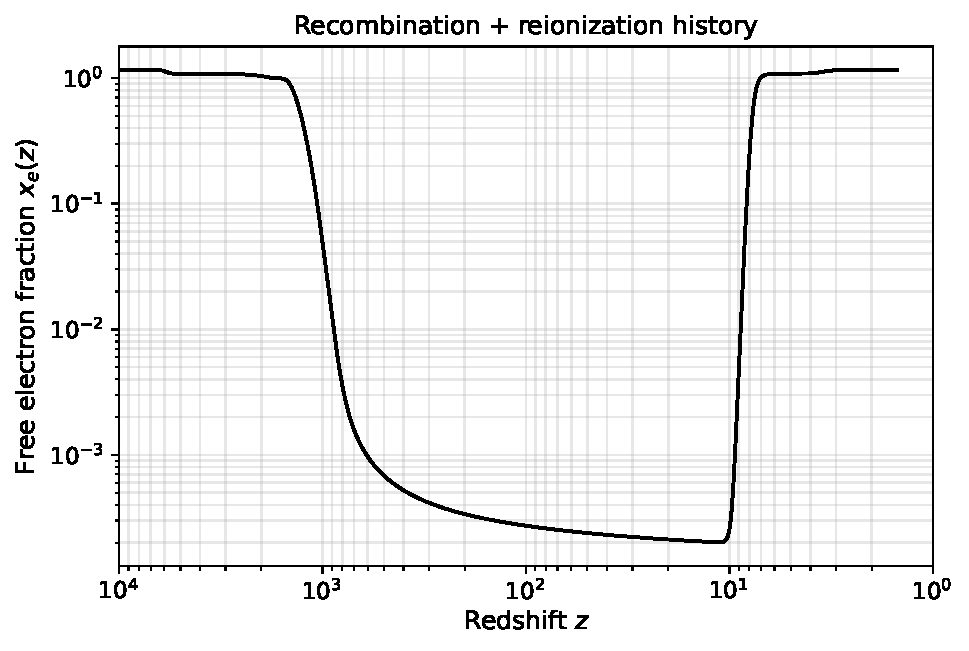
\includegraphics[width=0.85\linewidth]{figures/03_x_e_of_z.pdf}
\end{center}

Read this from right (high $z$) to left (low $z$): $x_e$ starts fully ionised ($\sim 1 + 2 f_\mathrm{He} \approx 1.16$), drops in two helium steps around $z \approx 6000$ and $z \approx 2500$ as He\textsuperscript{++} $\to$ He\textsuperscript{+} $\to$ He recombination completes, falls sharply through the main hydrogen recombination at $z \approx 1100$, plateaus at the freeze-out value $x_e \sim 10^{-4}$ through the cosmic dark ages, then jumps back to $\sim 1$ around $z \approx 7$ when reionisation kicks in.

\subsection{Plot: visibility function and Thomson opacity}

\begin{codebox}[Cell: plot $g(\tau)$ and $\dot\kappa(\tau)$]
\begin{lstlisting}[style=python]
fig, axes = plt.subplots(2, 1, sharex=True, figsize=(7, 6))
sel = th['tau_arr'] > 0
axes[0].semilogx(th['tau_arr'][sel], th['visibility'][sel], 'k-', lw=1.4)
axes[0].set_ylabel(r'Visibility $g(\tau)$')
axes[0].set_title('Visibility function and Thomson opacity')
axes[0].grid(True, which='both', alpha=0.3)
axes[1].loglog(th['tau_arr'][sel], th['opacity'][sel], 'k-', lw=1.4)
axes[1].set_ylabel(r'$\dot\kappa\, [\mathrm{Mpc}^{-1}]$')
axes[1].set_xlabel(r'Conformal time $\tau\, [\mathrm{Mpc}]$')
axes[1].grid(True, which='both', alpha=0.3)
plt.show()
\end{lstlisting}
\end{codebox}

\begin{center}
  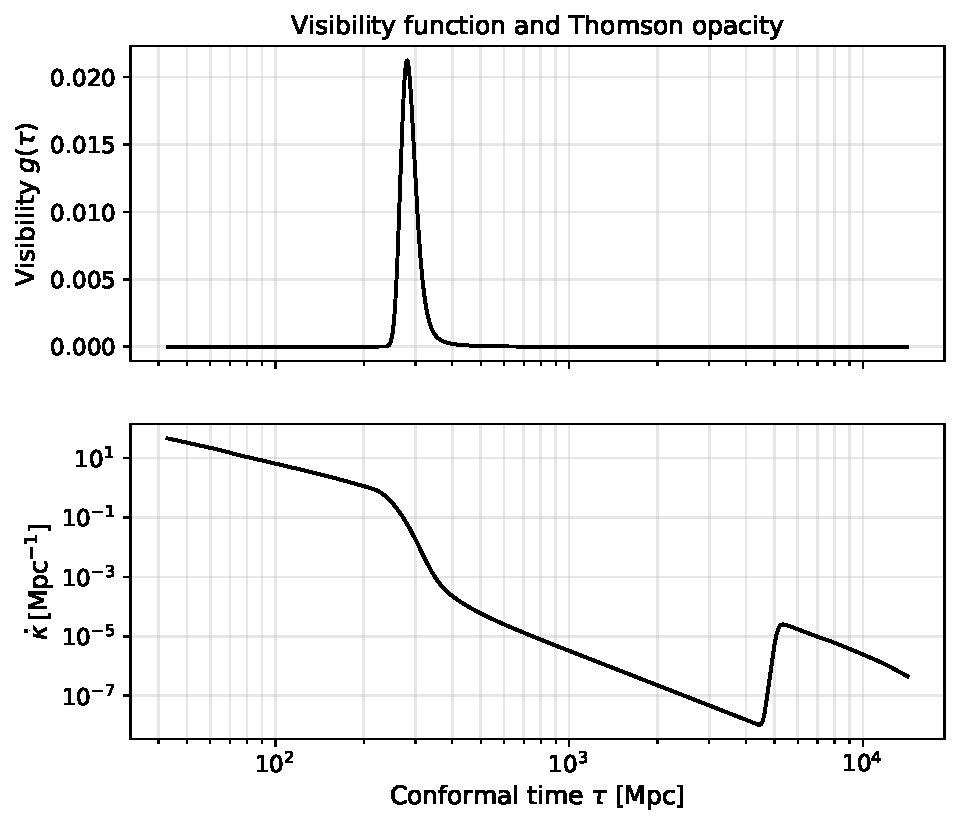
\includegraphics[width=0.85\linewidth]{figures/04_visibility_opacity.pdf}
\end{center}

The top panel shows $g(\tau)$ peaking sharply at $\tau_* \approx 281\,\mathrm{Mpc}$ -- the surface of last scattering -- with a small secondary bump around $\tau \approx 9000\,\mathrm{Mpc}$ from reionisation. The bottom panel shows the Thomson opacity $\dot\kappa$ dropping by about $12$ orders of magnitude across recombination as electrons leave the plasma, with a small late-time bump from reionisation.

\begin{physinsight}[Why recombination is sharp]
The visibility-peak width is set by the competition between recombination rate $\propto n_H \alpha^{(2)}$ and expansion rate $H$. Their ratio crosses unity exponentially fast because $\alpha^{(2)}$ varies as a low power of $T$ while photoionisation is exponentially suppressed by $e^{-B_H/T}$. The Saha-equation logic gives $\Delta T/T \sim T/B_H \sim 1/40$; converted to redshift, $\Delta z \approx z_*/40 \approx 30$. The full visibility function is somewhat wider ($\Delta z \approx 80$) because the freeze-out tail extends recombination. This narrowness is what makes ``last scattering'' an almost-well-defined surface.
\end{physinsight}

\subsection{Looking ahead}

The \texttt{th} dictionary now contains everything chapter 3 needs to evolve perturbations: the conformal-time grid \texttt{tau\_arr}, the opacity \texttt{opacity} (so we can compute Thomson scattering rates inside the Boltzmann hierarchy), the visibility \texttt{visibility} (for source functions in chapter 4), the baryon sound speed \texttt{cs2\_b} (for the baryon Euler equation), and the derived numbers $z_*$, $\tau_*$, $r_s$, $k_D$ that we will use to build optimal $k$- and $\tau$-grids.
